\documentclass[11pt]{article}

% ------- Packages -------
\usepackage[a4paper,margin=2.5cm]{geometry}
\usepackage{amsmath, amssymb}
\usepackage{physics}            % physics notation
\usepackage{graphicx}           % figures
\usepackage{caption}
\usepackage{subcaption}         % subfigures if needed
\usepackage{listings}           % code snippets
\usepackage{xcolor}             % colors for listings
\usepackage{hyperref}           % links and references
\usepackage[toc,page]{appendix} % appendices
\usepackage{siunitx}
\usepackage{enumitem}

% ------- Code listing settings -------
\lstset{
  language=Python,
  basicstyle=\ttfamily\footnotesize,
  keywordstyle=\color{blue},
  stringstyle=\color{orange},
  commentstyle=\color{gray},
  showstringspaces=false,
  breaklines=true,
  frame=single,
  captionpos=b,
  numbers = left,
  numberstyle = \tiny\color{gray},
}

% ------- Title -------
\title{Exam PUE Advanced Computational Physics}
\author{Jonas Bojanovsky, 12113264}
\date{\today}


\newcommand{\sub}[1]{_{\text{#1}}}
\newcommand{\super}[1]{^{\text{#1}}}




\begin{document}

\maketitle

\begin{abstract}
This paper presents a minimal example of a computational physics report with equations, code, and results. We simulate a basic physical system and analyze its behavior using numerical methods.
\end{abstract}

\section{Units and periodic boundary conditions}

We consider a Lennard Jones system with three particles. We have a quadratic box with side length $ L = \SI{12}{\AA} $

The three particles are at the positions:
\begin{align}
	\vec r_1 = \begin{pmatrix}
		1\\1\\1
	\end{pmatrix}\si{\angstrom}
\qquad
\vec r_2 = 
\begin{pmatrix}
	1\\1\\11
\end{pmatrix}
\si{\angstrom}
\qquad
\vec r_3
\begin{pmatrix}
	11\\11\\11
\end{pmatrix}\si{\angstrom}
\end{align}

Under the minimum image convention, we can implement a simple code to calculate the distances between the particles, implemented by the code
\begin{lstlisting}[language = Python, caption={Implementing Minimum image convention}]
 for i in range(3):
	if ri[i] - rj[i] > L / 2:
	rj[i] += L
	elif ri[i] - rj[i] < -L / 2:
	rj[i] -= L
	return rj - ri
\end{lstlisting}

Then, using $\vec r_1$ as the reference vector, we can find the center of mass in the minimum image convention, $\vec X$, by adding the MIC distances to $\vec r_1$ and averaging.	 This yields
\begin{equation}
	\vec X = \frac13 \begin{pmatrix} 1\\1\\-1\end{pmatrix}\si{\AA}
\end{equation}
Note that if we need to wrap it back into the original box, naturally this would become $\begin{pmatrix}1/3&1/3&35/3\end{pmatrix}\super{T}$.
With $\sigma = \SI{3.627}{\AA}$, the reduced center of mass is $\vec X^* = \vec X / \sigma$:
\begin{equation}
	\vec X^* = 0.0919\begin{pmatrix} 1 \\ 1 \\ -1\end{pmatrix}.
\end{equation}
And in the scaled coordinates, we instead scale by the length: $\vec X' = \vec X/L$:
\begin{equation}
	\vec X' = 0.0277 \begin{pmatrix} 1 \\ 1 \\ -1\end{pmatrix}.
\end{equation}

Calculating the potential energy, we use the contributions only from the three particles under the minimum image convention and do not consider the ones from other cells.
\begin{align}
	U_{12} &= 4919.11\varepsilon\\
	U_{13} &= 1.67\varepsilon\\
	U_{23} &= 61.30\varepsilon
\end{align}
The total sum of these contributions is
\begin{equation*}U = 4982.09\varepsilon.\end{equation*}.

\section{Parallel tempering MC simulation}

\subsection{Detailed balance for parallel tempering step}

A typical acceptance rule in the Metropolis step to preserve detailed balance is 
\begin{equation}
	p\sub{acc}(x\rightarrow y) = \min\left[1, \frac{f(y)}{f(x)}\right],
\end{equation}
where $y$ ($x$) is the new (old) sample from the ensemble and $f$ the corresponding probability density function.
For our case, 
\begin{equation}
	f(x) = \frac{1}{Q\sub{extended}}\prod_{k=1}^{M}\exp[-\beta_k H(x_k)]
\end{equation}
In our case, we just worry about the potential, so $H(x) = U(x)$.
In the trial step, we want to try to swap the positions from the trajectories from two different temperatures, $T_i$ and $T_j$.
So the swapped probability is:
\begin{equation}
	f(y) = \frac{1}{Q\sub{extended}}\exp[-\beta_j U(x_i)]\exp[-\beta_i U(x_j)]\prod_{k\neq i,j}\exp[-\beta_k H(x_k)]
\end{equation}
The ratio simplifies:
\begin{equation}\label{eq:acc}
	\frac{f(y)}{f(x)} = \exp\left[  (\beta_i - \beta_j) (U(x_i) - U(x_j)) = \exp[\Delta\beta\Delta U]      \right]
\end{equation}

In the exercise, however, the exponent is $-\Delta\beta\Delta U$. Our results agrees with \href{https://en.wikipedia.org/wiki/Parallel_tempering}{Wikipedia}.
We believe, however, that this is just an inconsistency in the definitions of $\Delta\beta$ and $\Delta U$, which we will continue to use exactly from the exercise sheet, but using the step with a positive exponent, as in \autoref{eq:acc}.

\subsection{Implementing the code}

The implementation of the potential can be seen in \autoref{ap:potential}.
The implementation of the MC with parallel tempering is in \autoref{ap:mcstep}.
The distributions of the trajectories with and without parallel tempering are in the figures \ref{fig:with} and \ref{fig:without} respectively.

\begin{figure}[p]
	\centering
	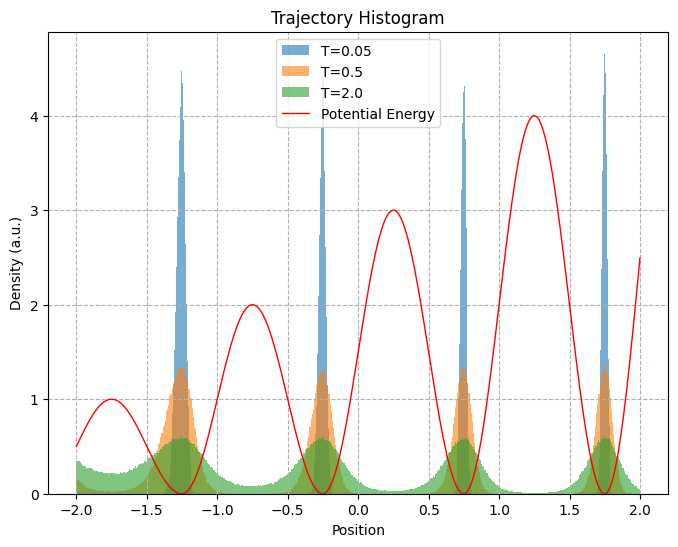
\includegraphics[width = 0.8\textwidth]{histogram_yes.png}
	\caption{Histogram of the particle position at different temperatures \textbf{with parallel tempering}. Potential only for visualization purposes, arbitrary units.}
	\label{fig:with}
\end{figure}
\begin{figure}[p]
	\centering
	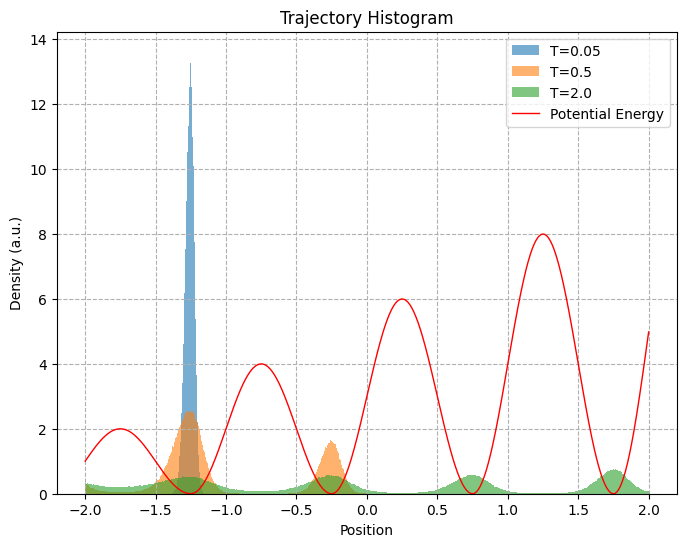
\includegraphics[width = 0.8\textwidth]{histogram_no.png}
	\caption{Histogram of the particle position at different temperatures \textbf{without parallel tempering}. Potential only for visualization purposes, arbitrary units.}
	\label{fig:without}
\end{figure}


The trajectory of the $ = 0.05$ particle at different zoom levels can be seen in Figures \ref{fig:all} -- \ref{fig:few}.

\begin{figure}[p]
	\centering
	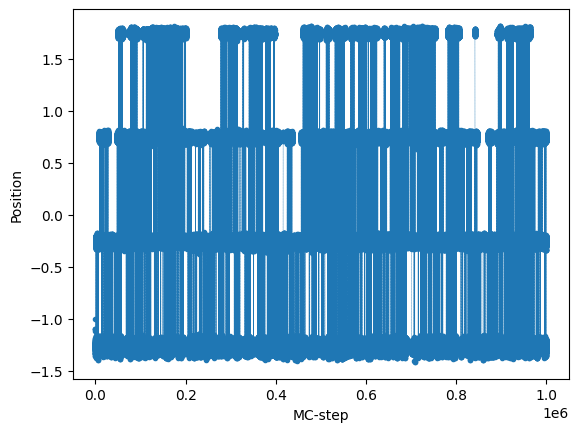
\includegraphics[width = 0.5\textwidth]{steps_all.png}
	\caption{position of $T = 0.05$ particle against time}
	\label{fig:all}
\end{figure}
\begin{figure}[p]
	\centering
	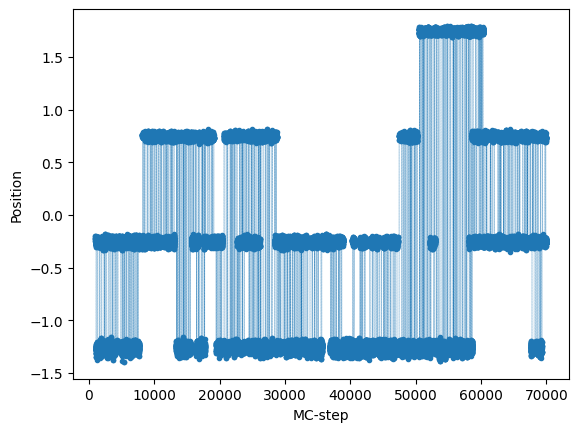
\includegraphics[width = 0.5\textwidth]{steps_many.png}
	\caption{position of $T = 0.05$ particle against time}
	\label{fig:many}
\end{figure}
\begin{figure}[p]
	\centering
	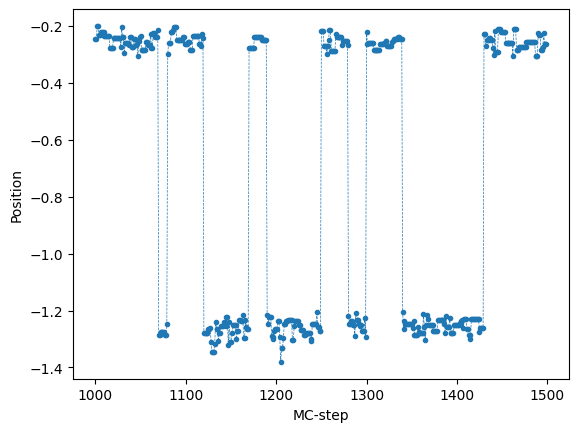
\includegraphics[width = 0.5\textwidth]{steps_few.png}
	\caption{position of $T = 0.05$ particle against time}
	\label{fig:few}
\end{figure}
\begin{figure}
	\centering
	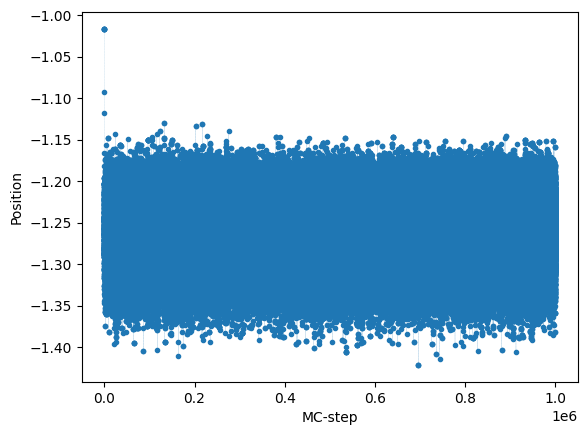
\includegraphics[width = 0.5\textwidth]{steps_no.png}
	\caption{position of $T = 0.05$ particle against time, no annealing}
	\label{fig:no}
\end{figure}

The simulation was run for $\num{1e6}$ steps. The acceptance ratio can be seen in \autoref{tab:acc}.

\begin{table}
	\centering
		\caption{Acceptance ratios (bottom two lines are the swapping acceptances for the tempering step)}
	\label{tab:acc}
	\begin{tabular}{r r r}\hline
		$T$ & tempering & no temp.\\\hline\hline
		0.05 & 0.37 & 0.46\\
		0.5 & 0.74 & 0.79\\
		0.2 & 0.88 & 0.89\\\hline
		$0.05 \leftrightarrow 0.5$ & 0.37 & -- \\
		$0.5 \leftrightarrow 2.0$ & 0.53 & --\\\hline\hline
	\end{tabular}

\end{table}

\subsection{Block averaging}

When estimating the standard error in the block averaging method, one tries to correct for the correlation in the samples by dividing the `trajectory' into blocks of size $B$ and calculating the variance of these averages. Note that there are $M = \lfloor N / B\rfloor$ blocks of this size, where $N$ is the number of simulation steps (in our case 1 Million).
Then the estimate for the true variance of the mean is
\begin{equation}
	(\Delta\bar x)^2 = \frac{1}{M(M-1)}\sum_{j=1}^M (\bar X_j - \langle x\rangle)^2,
\end{equation}
where $\langle x\rangle$ is the mean of the position (independent of the block size), and $\bar X_j$ is the position average of the $j\super{th}$ block.

To find the best possible estimate, one should calculate this for different block sizes and see where the computed value converges, while keeping the number of blocks $M$ large enough so that statistics is still meaningful.
In this simulation, this was not easy at all because sometimes, the values did not seem to converge at all, see \autoref{fig:converge}.

\begin{figure}
	\centering
	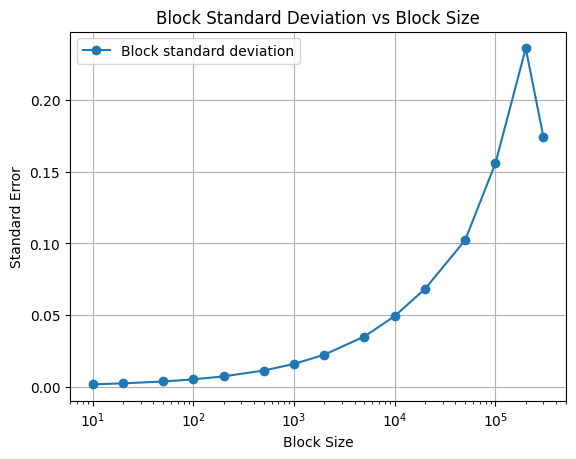
\includegraphics[width = 0.6\textwidth]{block_average.png}
	\caption{Standard error scaling with block size for $N =$ 1e6 steps, no annealing.}
	\label{fig:converge}
\end{figure}

Nevertheless, the estimated values can be found in \autoref{tab:averages}.
As a sanity check, we ran the simulation 10 times with tempering and recorded the average position each time. Then, computing the standard deviation of these averages should give a good estimate of the standard error, which is the deviation of the mean.
The results here agree well, as we get about $\Delta\bar x\sub{ann.} = 0.08$ for all temperatures, agreeing well with the estimate from the block-averaging method.
The values for the standard error in \autoref{tab:averages} was extracted by simply looking at the graphs and looking at convergence/local maxima and rounding up visually.


\begin{table}
	\centering
		\caption{Estimates for position averages and Standard errors with annealing (subscript `ann.') and without.}
	\label{tab:averages}
	\begin{tabular}{r r r r r}\hline
		T & $\langle x \rangle\sub{temp.}$ & $\Delta \bar x\sub{ann.}$ & $\langle x \rangle$ & $\Delta \bar x$\\\hline
		0.05 & 0.07 & 0.08 & -1.25 & \num{7e-5}\\
		0.5 & 0.02 & 0.07 & -0.96 & 0.25\\
		0.2 & -0.09 & 0.07 & -0.16 & 0.09\\\hline\hline
	\end{tabular}

\end{table}


\subsection{Discussion}

As expected from the histograms, the particles spend most of their `time' in the low-potential regions. Parallel tempering seems to be very effective to let the low-temperature trajectories explore local minima other than the one at -1.25, which is the one the system naturally falls into most likely due to the initial position $x = -1$.
Interestingly enough, in the tempering case, the particle spent slightly more time in the right-most minimum than the more left ones (this varied from run to run), probably because once it got there, due to the high maximum at $x = 1.25$, it could not get back so easily.

In the trajectories vs. time figures, one can clearly see how the particle jumps between the minima, showing the tempering process. In \autoref{fig:no}, where there is no tempering -- and especially at low temperature -- the particle just stays in the first minimum it falls into until the end of the simulation.

Note that at the beginning of the simulation there was an equilibration time, but after 100 steps the system was already equilibrated, so that this was sometimes just neglected, and sometimes the first 100 steps were thrown away when computing values, especially the averages.

The acceptance ratios of the MC steps get higher as the temperature increases -- as expected. Interestingly, for $T = 0.05$, the tempering case is significantly lower than the no-tempering case. This is likely due to the fact that, when swapping with the higher-temperature particle, there are more `forbidden' regions, and the particle in the no-tempering case justs sits in its local minimum comfortably, which is locally relatively flat.

In the tempering case, the $\langle x\rangle$ move to the left with higher temperature. This is probably due to the minimum at -2, which become more accessible to higher-temperature particles, but the other ones at $U = 0$ potential are due to tempering equally accessible to all particles.
On the other hand, the no-tempering averages move to the right with higher temperature, because only the higher-temperature particles ever overcome the higher and higher barriers to the right.

An outlier in the standard error is the no-tempering, $T = 0.05$ case. Because it very securely sits in the -1.25 minimum, it is extremely well localized there, hence the low $\Delta\bar x$.






\newcommand\mean[1]{\left\langle#1\right\rangle}


\section{Exponential correlations}

From the ACOMP script we know that $\text{MSD} \equiv \langle[r(t) - r(0)]^2\rangle$ is related to the VACF by
\begin{align}
	\text{MSD} &= 2\cdot \int_0^t \dd{t'} \int_0^{t'} \dd{t''} \mean{v(0) v(t'')}\\
	&= 2\cdot \int_0^t \dd{t'} \mean{v^2} \tau\left(1-e^{-t'/\tau}\right)\\
	&= 2 \mean{v^2} \tau\left[t - \tau\left(1-e^{-t/\tau}\right)\right]
\end{align}

Similarly, we can get the diffusion coefficient $D$:
\begin{align}
	D &= \frac13\int_0^\infty \dd{t} \mean{v(0)v(t)}\\
	\Rightarrow D &= \frac13 \mean{v^2} \tau \label{eq:D}
\end{align}

Further, if we expand the MSD, we get
\begin{align}
	&2\mean{v^2}\left[\tau t - \tau^2 \left(1-1-\frac t\tau - \frac{t^2}{2\tau^2} - O(t^3)\right)\right]\\
	= &2\mean{v^2}t^2 + O(t^3).
\end{align}

So for small t, the system behaves balistically (MSD scales with $t^2$).
On the other hand, for $t\rightarrow\infty$  (same as $\tau\rightarrow 0$), we get
\begin{equation}
	\text{MSD} \rightarrow 2\mean{v^2}\tau t = 6Dt,
\end{equation}
which is consistent with theory, and is diffusive motion.
So $\tau$ is like a relaxation or diffusion time, how long the system `remembers' it's original velocity, i.e. stays in the ballistic regime before transitioning to the diffusive one.

For water, we assume $D = \SI{31e-5}{cm^2/s}$. From the Boltzmann distribution we know that
\begin{equation}
	\mean{v^2} = \frac{3 k\sub B T}{m},
\end{equation}
where $m \approx \SI{18}{amu} = \SI{3e-26}{kg}$.
From that we get $\mean{v^2} = \SI{4.16e9}{cm^2/s}$.
Now, using \autoref{eq:D}, we get
\begin{equation*}
	\tau = \SI{22}{fs}.
\end{equation*}










\section{Judging results}

\begin{enumerate}[wide]
	\item Energy in the NVE ensemble should be (almost) perfectly constant, but here it increases.
	\item Sudden step in potential energy hints at a melting process, or at least some breaking of the FCC structure, which is completely ignored. This would be consistent with the parameters, because at $T  = 1.5$ and $\rho^* = 0.8$ there should be gas phase for an LJ system, at least definitely not solid.
	\item There is no plot of the kinetic energy, why?
	\item There is no mention of the time step used, which is critical to examine stability, especially for integrators like Euler-forward.
	\item Euler forward is a really bad integrator for energy conserving simulations. A symplectic integrator like velocity-verlet should be implemented instead.
	\item 30 particles really is not many for such a system and finite-size effects may play a role, but it is completely ignored.
	\item The temperature plot is completely missing from this, although it should not be expected to stay constant.
	\item Is there a cutoff radius in the simulation? We use periodic boundary conditions. The cutoff radius may also be difficult.
\end{enumerate}

Based on these issues, especially the ignoring of the melting, missing information about the time step and bad choice of integrator, I would not trust these results or the speaker that they really knew what they were doing.



\newpage
\begin{appendices}
\section{Defining Potential and quantities} \label{ap:potential}
\begin{lstlisting}[language=Python, caption={Defining the potential and fixed quantities}]
def U(x):
	"""Potential"""
	U = 1 + np.sin(2 * np.pi * x)
	
	if x < -2 or x > 2:
	return np.inf
	elif -1.25 <= x <= -0.25:
	U *= 2
	elif -0.25 <= x <= 0.75:
	U *= 3
	elif 0.75 <= x <= 1.75:
	U *= 4
	elif  1.75 <= x <= 2:
	U *= 5
	return U
	
	
	Temperatures = np.array([0.05, 0.5, 2.0]) # k_B = 1
	betas = 1/Temperatures
	
	x_initial = -1.0
	
	maximum_displacement = 0.1
	
	parallel_tempering_after = 10
	
\end{lstlisting}

\section{Metropolis MC algorithm with parallel tempering}\label{ap:mcstep}
\lstinputlisting[language=Python]{metropolisstep.py}



\end{appendices}




\end{document}


